\documentclass[parskip=full,11pt]{scrartcl}

\usepackage[sfdefault,light]{roboto}
\usepackage{inconsolata}
\usepackage[english]{babel}

\usepackage[utf8]{inputenc}
\usepackage[T1]{fontenc}

\usepackage{microtype}

\usepackage{csquotes}
\MakeOuterQuote{"}

\usepackage{graphicx}
\usepackage{float}
\usepackage{bm}
\usepackage{amssymb}
\usepackage[hidelinks]{hyperref}
\usepackage[section]{placeins}


\usepackage[T1]{fontenc}
\usepackage[scaled=0.85]{beramono}

%circled numbers
\usepackage{tikz}
\newcommand*\circled[1]{\tikz[baseline=(char.base)]{
            \node[shape=circle,draw,inner sep=2pt] (char) {#1};}}

%embed small pngs into text lines
\usepackage{calc}
\newlength\myheight
\newlength\mydepth
\settototalheight\myheight{Xygp}
\settodepth\mydepth{Xygp}
\setlength\fboxsep{0pt}
\newcommand*\inlinegraphics[1]{%
  \settototalheight\myheight{Xygp}%
  \settodepth\mydepth{Xygp}%
  \raisebox{-1.8\mydepth}{\includegraphics[height=1.75\myheight]{#1}}%
}


\begin{document}
\begin{titlepage}
	\centering
	\vspace*{5cm}
	
\includegraphics[width = 0.7\linewidth]{img/logo.png}\par
	{\huge\bfseries A simulator for  repeated games\par}
	%\vspace{1cm}
	{\Large Manual\par}
\end{titlepage}

\tableofcontents
\pagebreak

\section{Introduction}
This program is designed for scientific research in the field of game theory. 

\section{Getting started}
When the program is first started, the home window will show as in Fig. \ref{fig:program_start}. Since no simulations have been executed yet, it is mostly empty.

The home window is roughly divided into three areas. In the top area, a short summary of the currently active configuration is displayed (\circled{1} in Fig.\ref{fig:program_start}). If the user hasn't created a configuration of his own yet, a predefined one will be active. On the right-hand side of the summary reside two buttons (\circled{2} and \circled{3}). The one labeled with a cog symbol opens up the configuration window, in which the currently active configuration can be modified (see \ref{sec:edit_config}). Pressing the Play-button will start a simulation with the currently active configuration. The left-hand side area (\circled{4} in Fig.\ref{fig:program_start}) will contain a list of all running, finished and cancelled simulations. If a finished simulation is selected, detailed information about its results will be displayed in area \circled{5} (This area will from now on be referred as the \enquote{output view}).

\begin{figure}
	\centering
	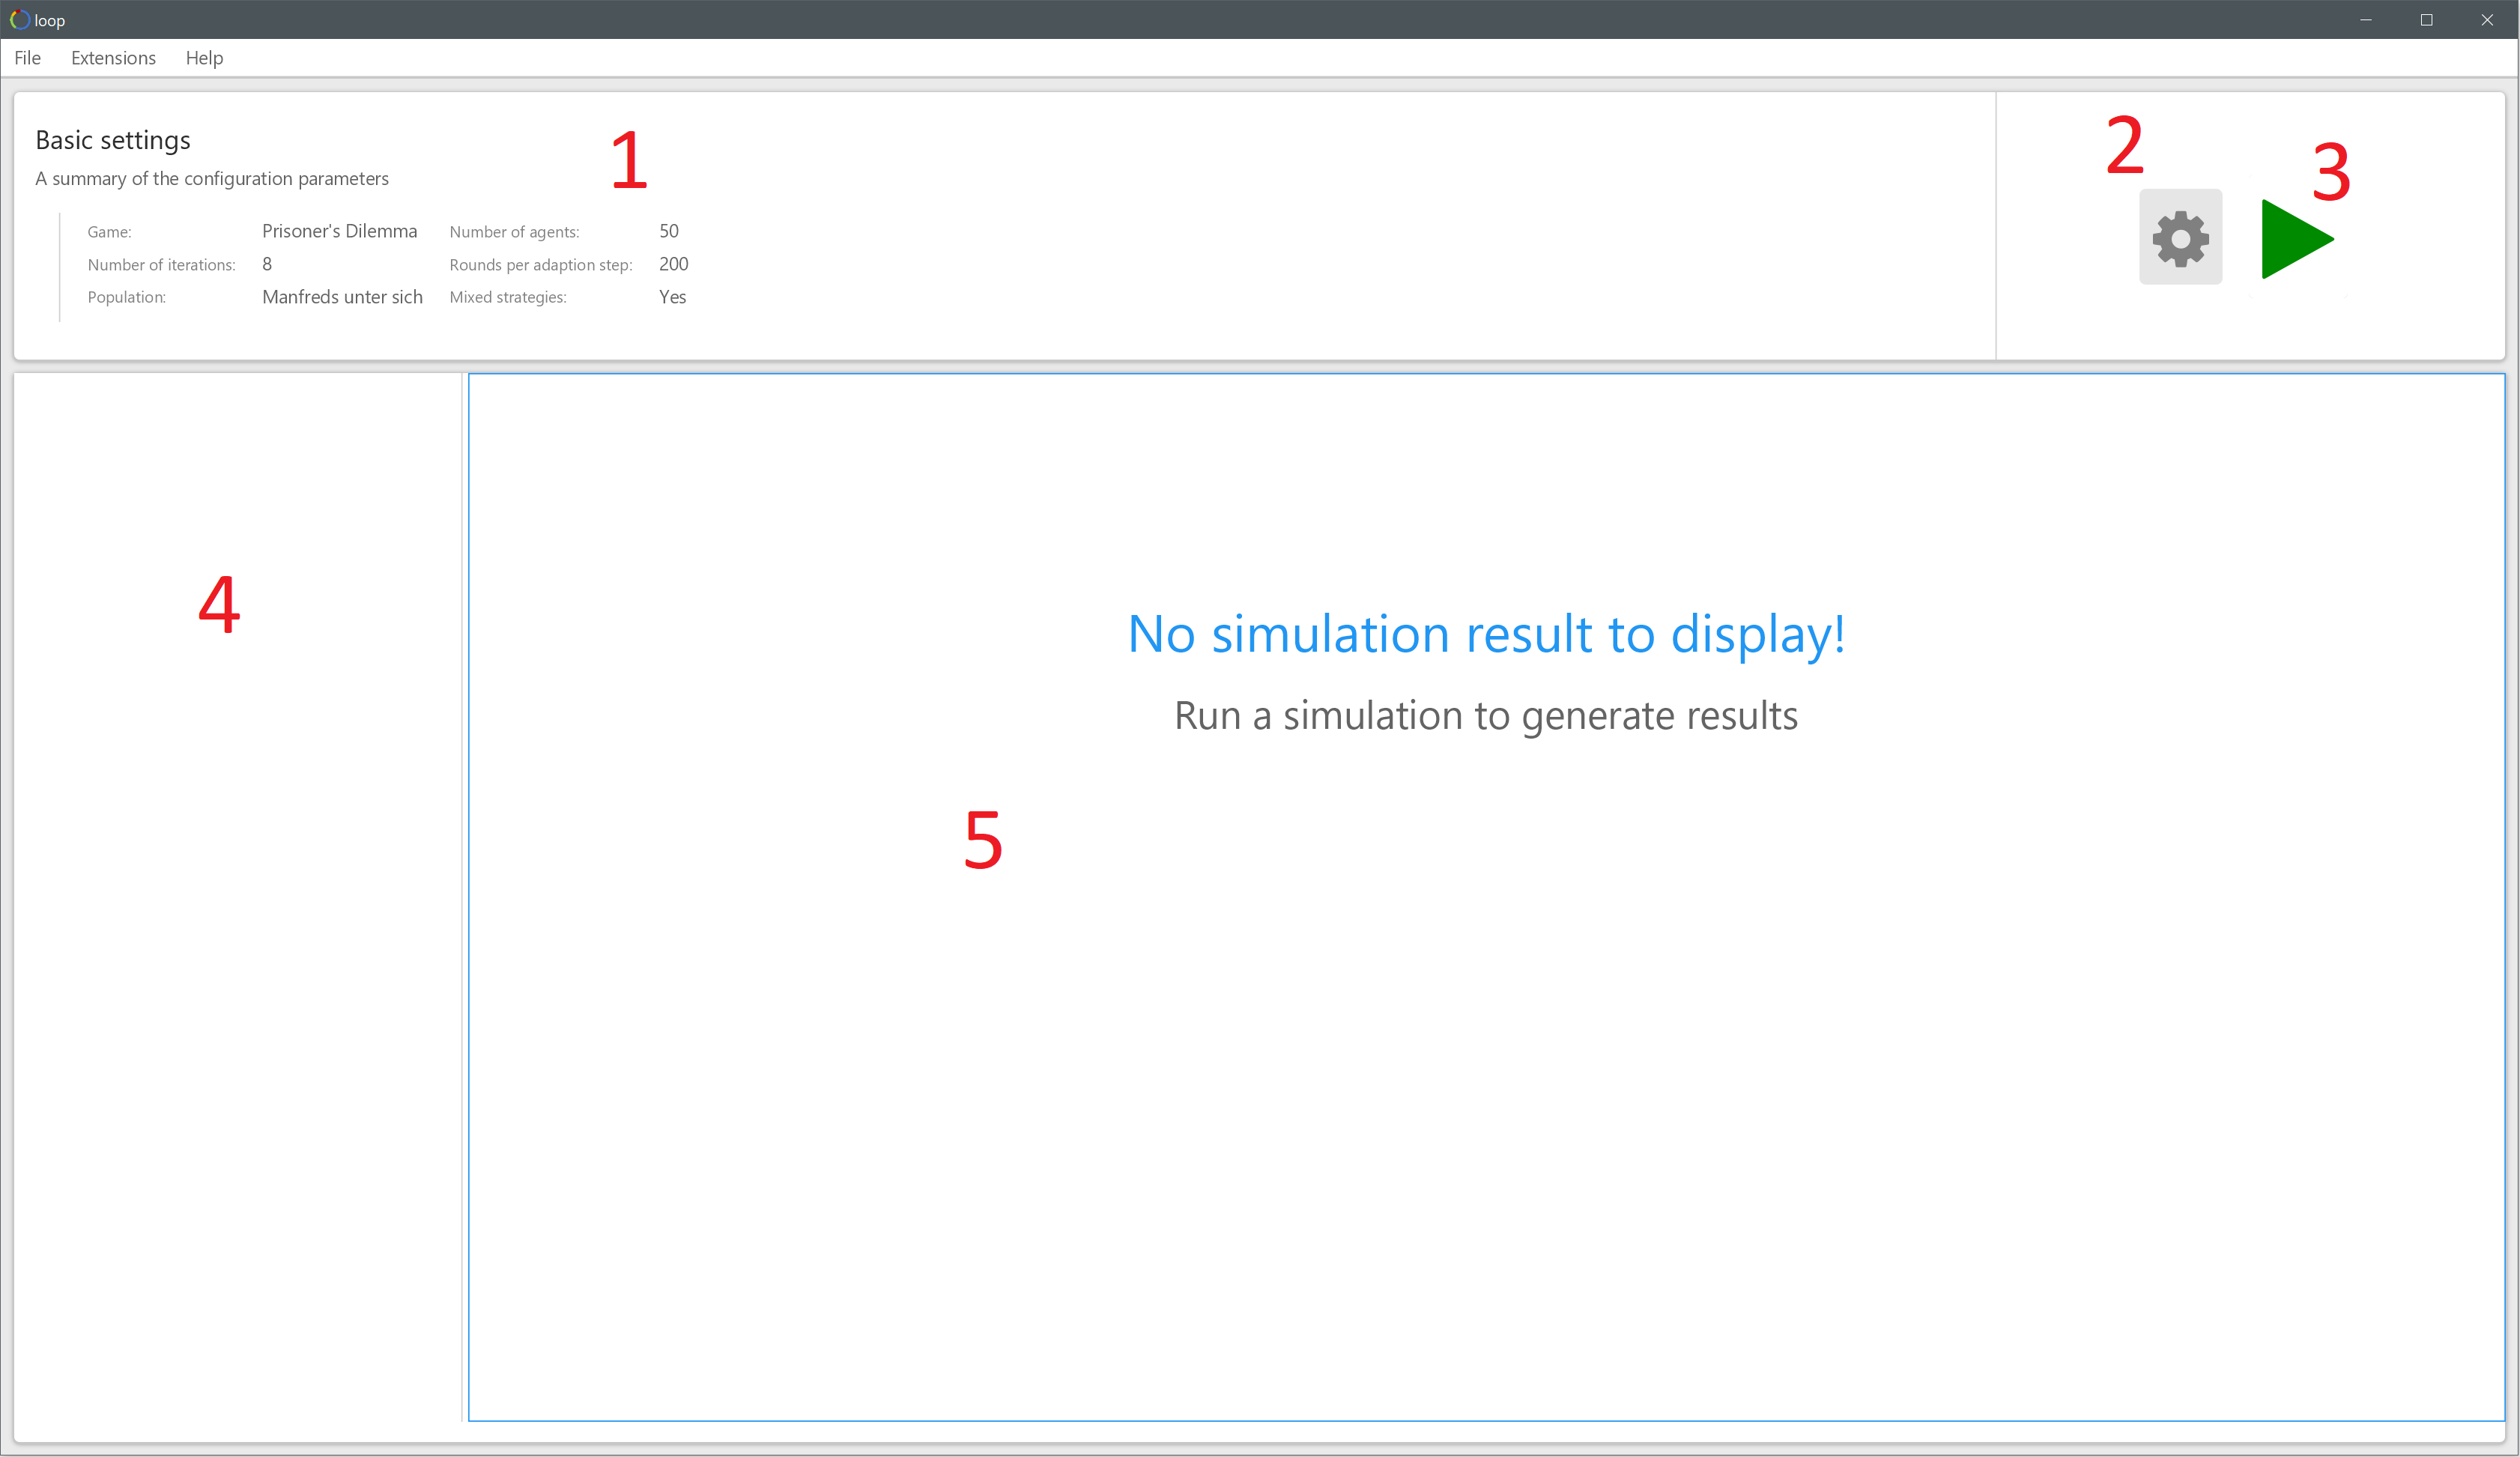
\includegraphics[width=\linewidth]{img_manual/program_start.png}
	\caption{The home window after the first start of the program.}
	\label{fig:program_start}
\end{figure}

\subsection{Edit the configuration}\label{sec:edit_config}
To edit the active configuration, press the cog-labeled button in the home window. This will open up the configuration window (see Fig.\ref{fig:config_window}). On the left-hand side, all configurable parameters of a simulation can be modified. If the selected pairing algorithm, success quantification, strategy adaption mechanism or equilibrium criterion has configurable parameters, they can be entered below the corresponding dropdown menu (see \circled{1} in Fig.\ref{fig:config_window}). On the right-hand side, a short description and a table containing the payoffs of the selected game are displayed (see \circled{2} in Fig.\ref{fig:config_window}). Below (\circled{3} in Fig.\ref{fig:config_window}), a multiconfiguration can be activated, see section \ref{?}.

The  \inlinegraphics{img_manual/rotate_left_button.png} - button will reset all settings to the default configuration. Pressing the  \inlinegraphics{img_manual/check_button.png} - button will close the configuration window and apply the made changes to the active configuration.

\begin{figure}
	\centering
	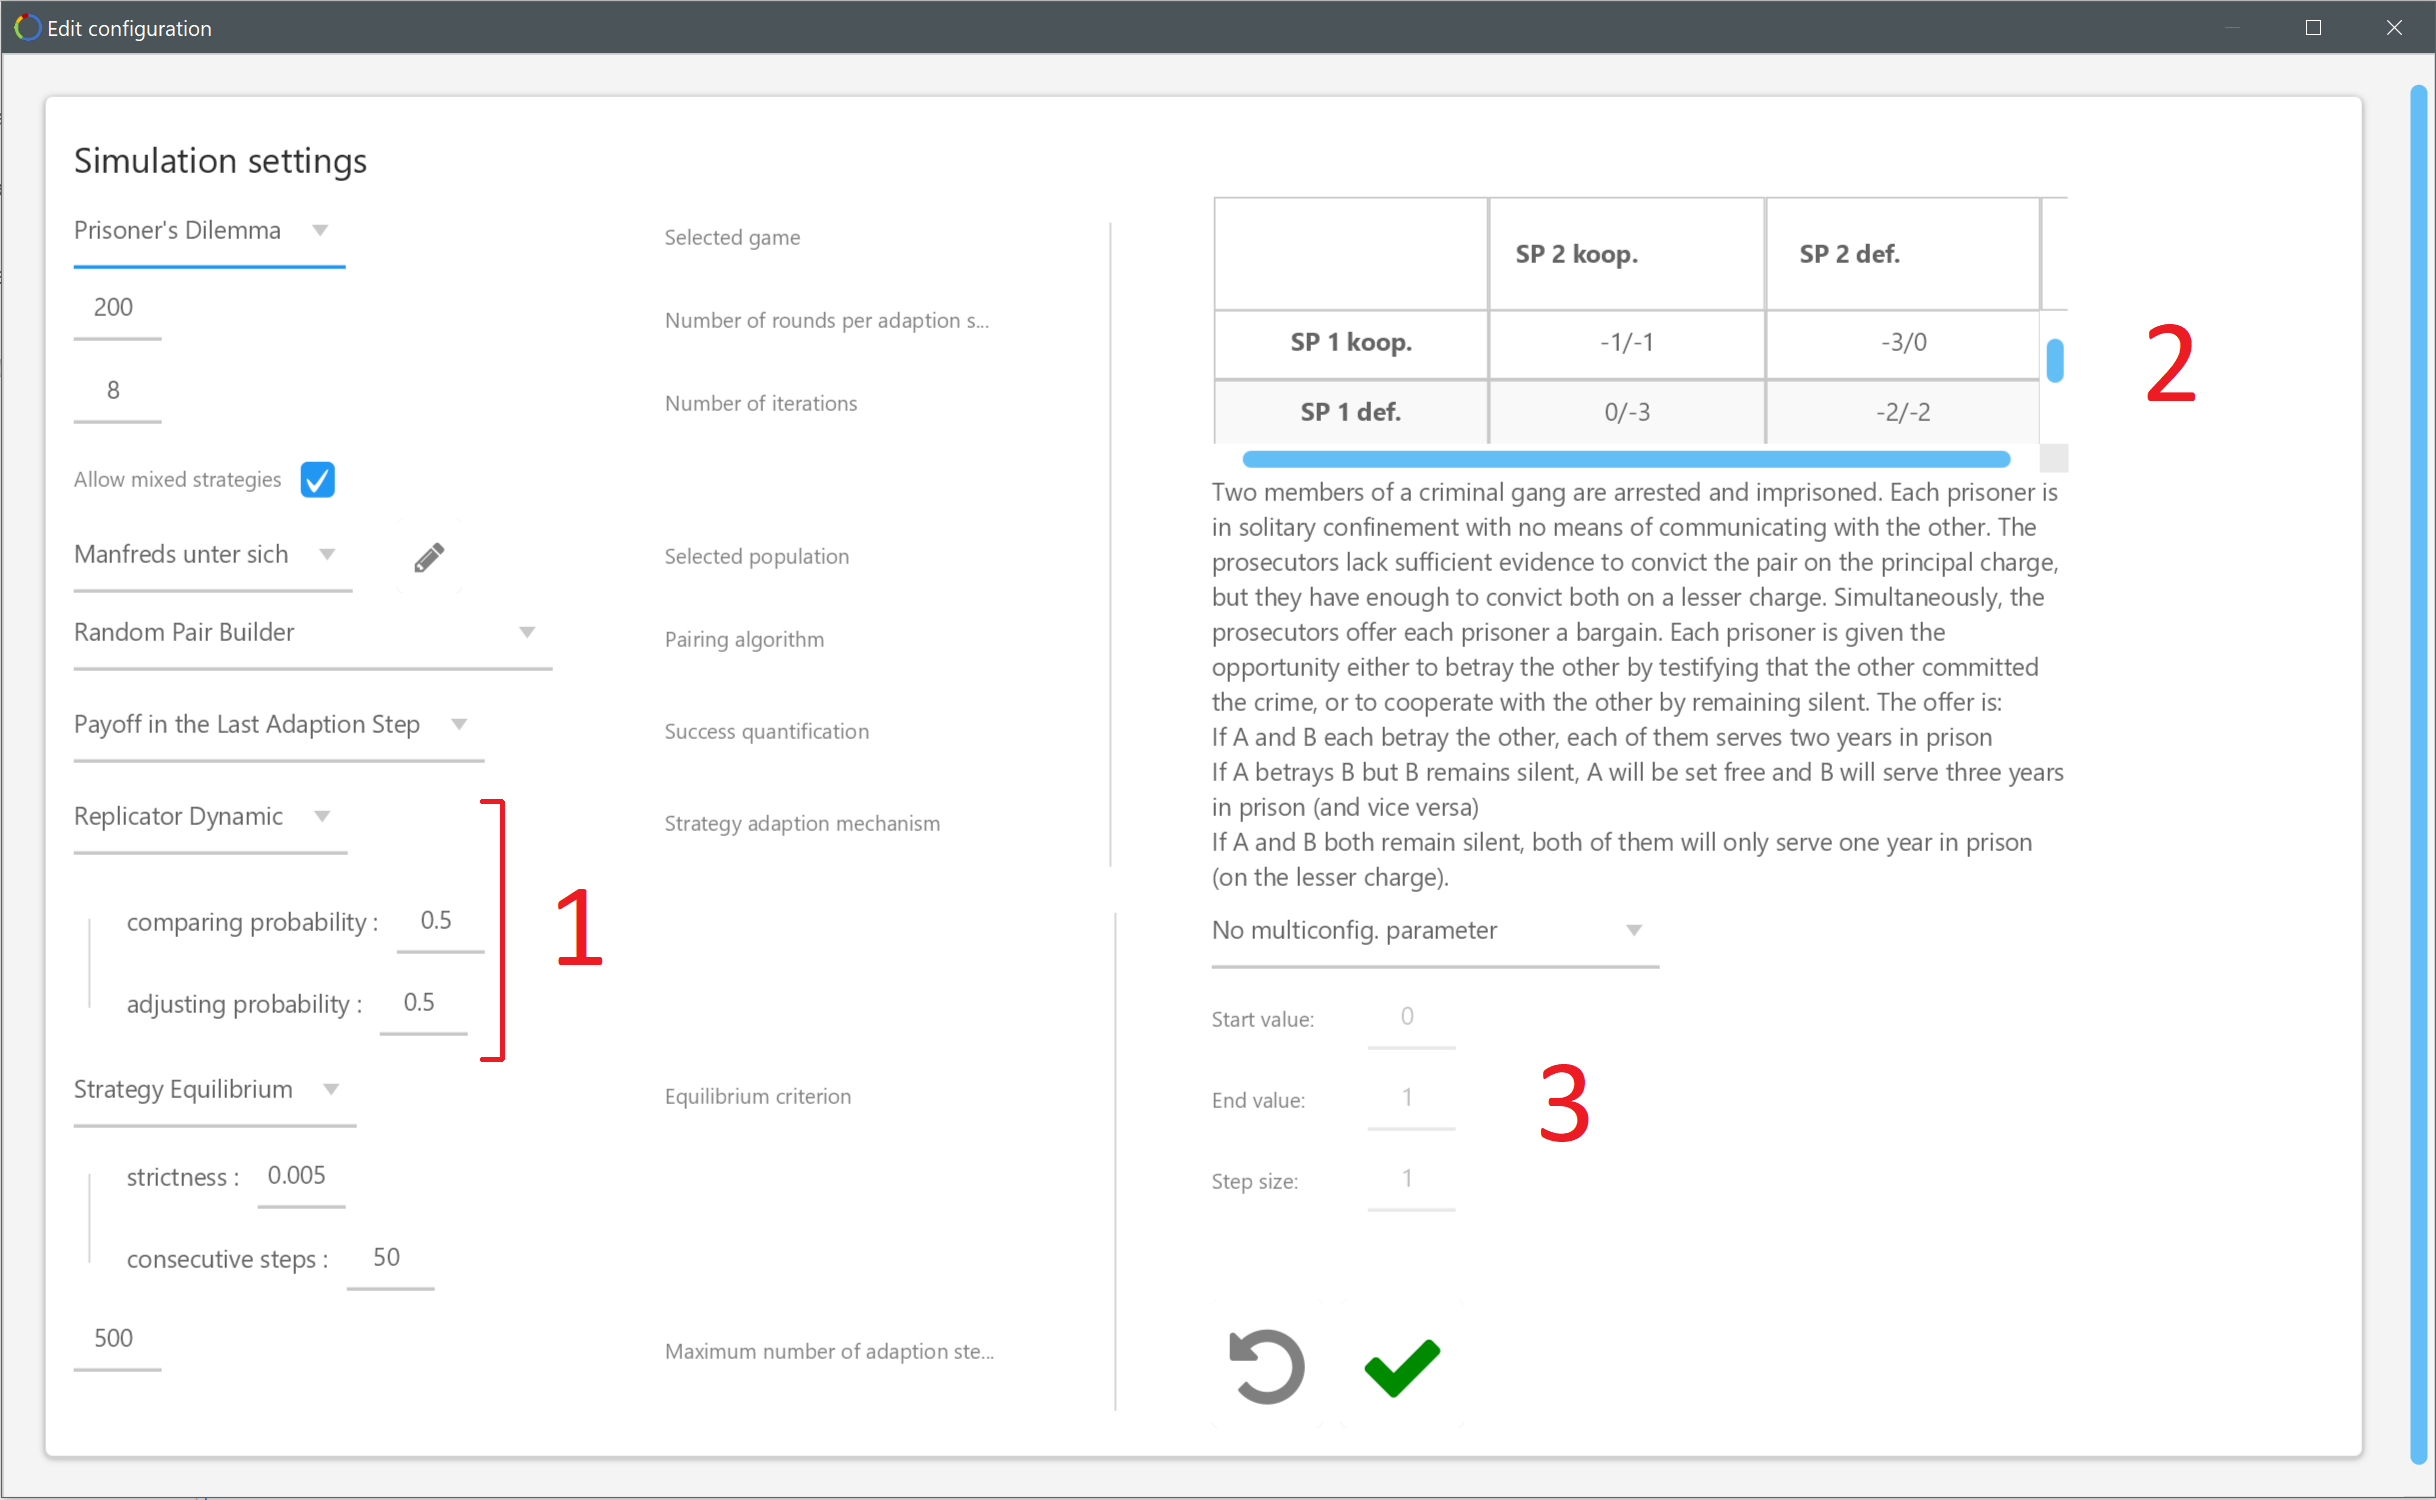
\includegraphics[width=\linewidth]{img_manual/config_window.png}
	\caption{The configuration window.}
	\label{fig:config_window}
\end{figure}

\subsection{Start a simulation}
Pressing the Play-button in the home window will start a simulation with the currently active configuration. It will then appear in the list in the left-hand side area of the home window. The list entry displays an estimate for the time left until the simulation is finished as well as how many iterations have already been executed. If the running simulation is selected, the output view will contain the same information as the list entry as well as a button labeled with an  \inlinegraphics{img_manual/x_button.png}. If pressed, the simulation is cancelled.

\begin{figure}
	\centering
	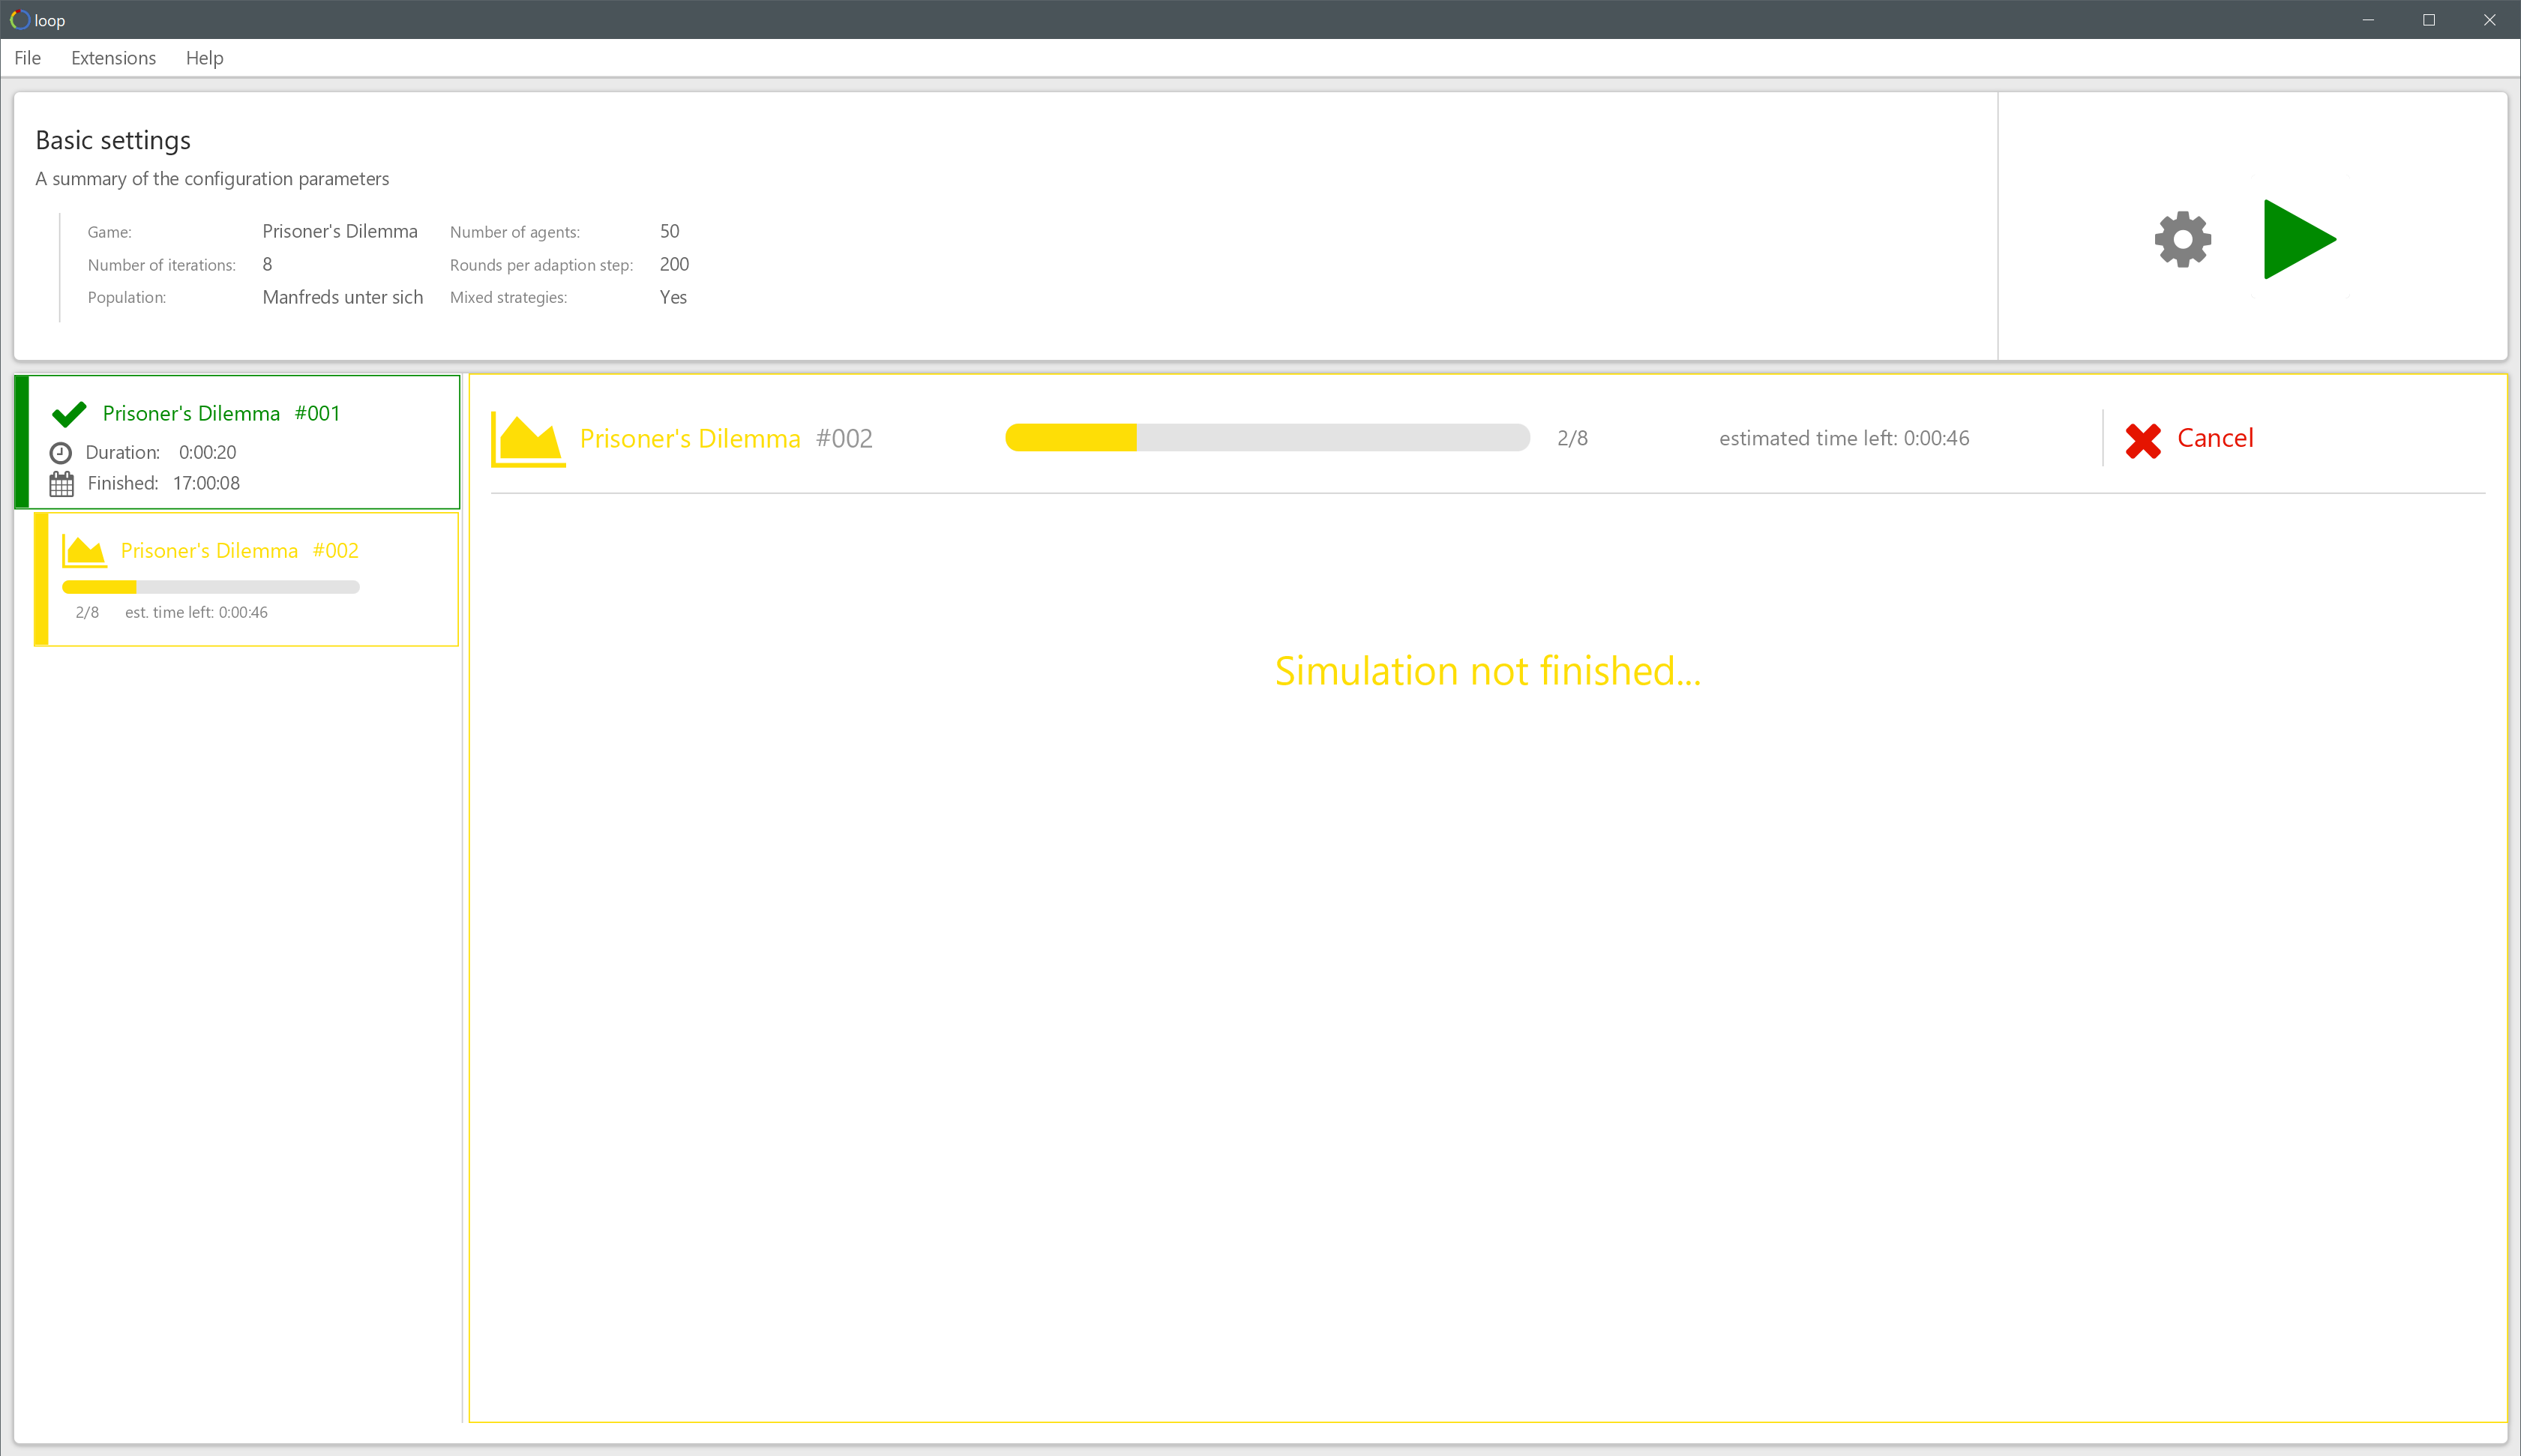
\includegraphics[width=\linewidth]{img_manual/running_simulation.png}
	\caption{The home window with a running simulation selected.}
	\label{fig:running_simulation}
\end{figure}

\subsection{View the simulation results}


\end{document}